\documentclass[a4paper]{article}

%% Language and font encodings
\usepackage[english]{babel}
\usepackage[utf8x]{inputenc}
\usepackage[T1]{fontenc}

%% Sets page size and margins
\usepackage[a4paper,top=3cm,bottom=2cm,left=3cm,right=3cm,marginparwidth=1.75cm]{geometry}

%% Useful packages
\usepackage{amsmath}
\usepackage{graphicx}
\usepackage[colorinlistoftodos]{todonotes}
\usepackage[colorlinks=true, allcolors=blue]{hyperref}
\usepackage{scrextend} % lists
\usepackage{float}
\addtokomafont{labelinglabel}{\bfseries}

\title{Music recomendation}
\author{Raquel Leandra Pérez Arnal i Adrián Sánchez Albanell}
\date{} % Sin fecha.

\begin{document}
\maketitle
\clearpage
\tableofcontents
\clearpage

\section{Descripción del trabajo}


\subsection{Introducción}
Este trabajo consiste en elegir un problema de regresión o clasificación y generar un modelo para resolverlo. Para ello usaremos algunos de los métodos, lineales y no lineales, vistos en clase durante el curso de Aprendizaje Autónomo.\\
Hemos elegido un problema de \href{https://www.kaggle.com/competitions}{kaggle competitions} sobre recomendación de música llamado \href{https://www.kaggle.com/c/kkbox-music-recommendation-challenge}{WSDM - KKBox's Music Recommendation Challenge}. Este consiste en un dataset, proporcionado por \href{https://www.kkbox.com/intl/index.php?area=intl}{KKBOX} - servició de streaming de música asiático - con información sobre diferentes canciones, usuarios y como ha sido el acceso de los usuarios a dichas canciones.\\
El objetivo es predecir si un usuario que ha escuchado una canción lo volverá a hacer en un periodo de tiempo determinado, por lo tanto se trata de un problema de clasificación binaria: si el usuario volverá a escuchar o no una canción que ya ha oído anteriormente.


\subsection{Conjunto de datos disponible}
Kaggle nos ha proporcionado los datos en seis ficheros CSV, de los cuales usaremos cuatro para la práctica.Los dos restantes són un conjunto de datos de muestra sobre como enviar los datos para el concurso y los datos de test para el concurso (que no nos sirven ya que vienen sin la variable target).

\subsection*{train.csv}
Contiene la información de las reproducciones de canciones por parte del usuario. Tiene las siguientes variables:
\begin{labeling}{source\_screen\_name}
\item [msno] identificador del usuario.
\item [song\_id] identificador de la canción.
\item [source\_system\_tab] nombre de la pestaña donde se selecciono el evento.\\ Ejemplos: \textit{my library}, \textit{search}, etc.
\item [source\_screen\_name] nombre de la pantalla que ve el usuario.
\item [source\_type] des de donde se ha reproducido la canción.\\ Ejemplos: \textit{album}, \textit{online-playlist}, \textit{song}, etc.
\item [target] variable de target. Si el usuario ha escuchado la canción más de una vez en un intervalo de un mes target es 1, si no es 0.
\end{labeling}

\subsection*{members.csv}
Contiene información de los usuarios. Tiene las siguientes variables:
\begin{labeling}{registration\_init\_time}
\item [msno] identificador del usuario.
\item [city] identificador de ciudad.
\item [bd] edad del usuario. Contiene valores outlier.
\item [gender] genero del usuario. Puede ser \textit{female} o \textit{male}.
\item [registered\_via] identificador del método de registro de usuario.
\item [registration\_init\_time] día del registro de usuario, en formato \textit{\%Y\%m\%d}.
\item [expiration\_date] día de expiración del registro de usuario, en formato \textit{\%Y\%m\%d}.
\end{labeling}

\subsection*{songs.csv}
Tiene tamaño: (2,286,220 , 7)

Contiene información de las canciones. Tiene las siguientes variables:
\begin{labeling}{song\_length}
\item [song\_id] identificador de la canción.
\item [song\_length] duración de la canción en milisegundos.
\item [genre\_ids] género musical de la canción. Hay canciones con más de un genero, donde el carácter | hace de separador.
\item [artist\_name] nombre del artista.
\item [composer] nombre del compositor o compositores. Si hay más de uno el carácter | hace de separador.
\item [lyricist] nombre del escritor o escritores de la canción. Si hay más de uno el carácter | hace de separador.
\item [language] identificador del lenguaje de la canción.
\end{labeling}

\subsection*{song\_extra\_info.csv}
Contiene información extra de las canciones. Tiene las siguientes variables:
\begin{labeling}{song\_name}
\item [song\_id] identificador de la canción.
\item [song\_name] nombre de la canción.
\item [isrc] \href{https://en.wikipedia.org/wiki/International_Standard_Recording_Code}{International Standard Recording Code}. En teoría se puede usar como identificador de la canción, pero hay codigos ISRC sin verificar. Contiene información de la canción aunque puede ser erronea o confusa como el country code, que no se refiere a la canción si no a la agencia que proporciona el codigo ISRC.
\end{labeling}


\subsection{Notas sobre el lenguaje de programación escogido}


\section{Trabajo Relacionado}


%\section{Posibles Métodos}
%\begin{itemize}
%\item logistic regression, multinomial regression
%(single-layer MLP), LDA, QDA, RDA, \textbf{Naive Bayes}, \textbf{nearest-neighbours},\textbf{linear SVM}, quadratic SVM
%\item one-hidden-layer MLP, the RBFNN, the SVM with RBF kernel, a
%Random Forest
%\end{itemize}


\section{Data exploration and Preprocessing}

Los datos iniciales son: 
\begin{itemize}
\item train.csv
\item test.csv
\item songs.csv
\item members.csv
\item song\_extra\_info.csv
\end{itemize}

La idea inicial es mejorar train utilizando songs, members y song\_extra\_info y convertirlo en un único train y test. 

Después pasar todas las variables categóricasa numéricas y aplicarle un MCA.

Debería quedar: 
\begin{itemize}
\item clean\_train.csv
\item clean\_test.csv
\end{itemize}


\subsection{Selección de features}

Eliminamos las siguientes variables por los siguientes motivos


\begin{table}[H]
\centering
\caption{My caption}
\label{my-label}
\begin{tabular}{|l|l|}
\hline
Nombre                   & Motivo \\ \hline
msno                     & Es solo un identificador \\ \hline
song\_id                 & Es solo un identificadors \\ \hline
artist\_name             & Computacionalmente intratable \\ \hline
composer                 & Computacionalmente intratable \\ \hline
lyricist                 & Computacionalmente intratable    \\ \hline
name                     & Computacionalmente intratable     \\ \hline
isrc                     & Es solo un identificador    \\ \hline
\end{tabular}
\end{table}


\subsection{Tratamiento de valores perdidos}


\begin{figure}[H]
\centering
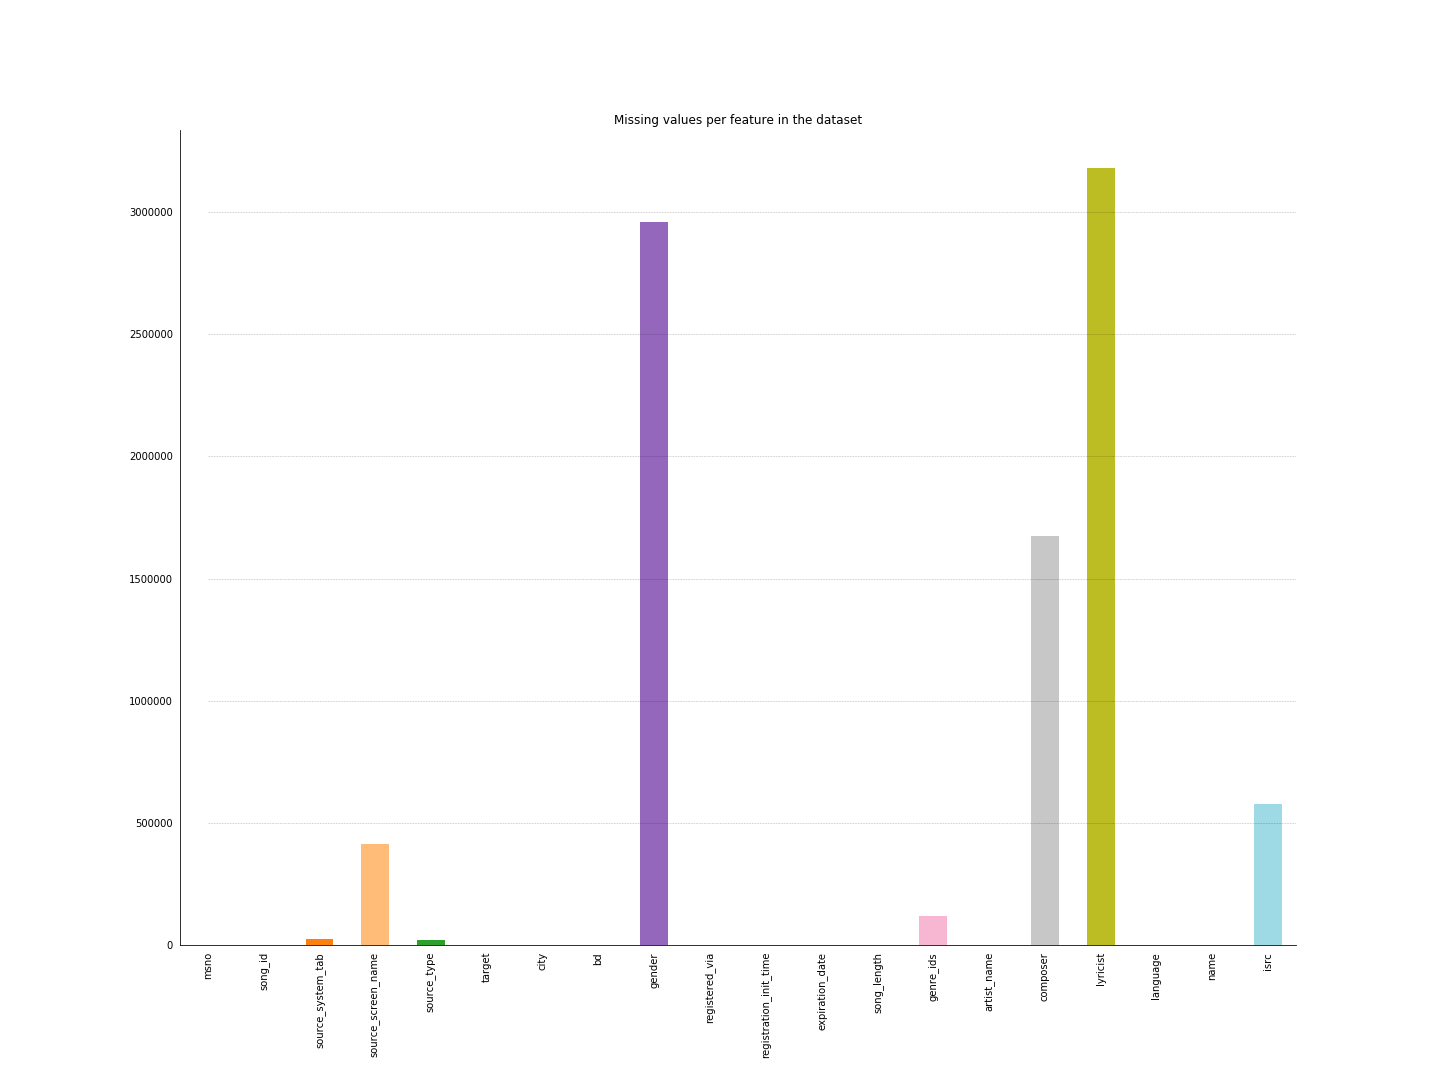
\includegraphics[width=1\textwidth]{Images/missings.png}
\caption{En esta gráfica podemos ver la cantidad de valores perdidos que tiene el conjunto de datos final}
\end{figure}

\begin{table}[H]
\centering
\caption{My caption}
\label{my-label}
\begin{tabular}{|l|l|}
\hline
Nombre                   & Porcentage \\ \hline
msno                     & 0          \\ \hline
song\_id                 & 0          \\ \hline
source\_system\_tab      & 0.3368     \\ \hline
source\_screen\_name     & 5.6226     \\ \hline
source\_type             & 0.2919     \\ \hline
target                   & 0          \\ \hline
city                     & 0          \\ \hline
bd                       & 0          \\ \hline
gender                   & 40.142     \\ \hline
registered\_via          & 0          \\ \hline
registration\_init\_time & 0          \\ \hline
expiration\_date         & 0          \\ \hline
song\_length             & 0.0015     \\ \hline
genre\_ids               & 1.605      \\ \hline
artist\_name             & 0.0015     \\ \hline
composer                 & 22.7139    \\ \hline
lyricist                 & 43.0882    \\ \hline
language                 & 0.0020     \\ \hline
name                     & 0.0197     \\ \hline
isrc                     & 7.8327     \\ \hline
\end{tabular}
\end{table}


Viendo esta información descartamos \textit{lyricist} y \textit{composer}

En el resto de variables eliminamos las muestras con missings salvo en \textit{gender}. 

\textbf{Tratamiento de los valores perdidos en \textit{gender}}.

Los imputamos utilizando la clasificación que nos daría un knn.

\subsection{Tratamiento de outliers}

\subsection{Tratamiento de valores incorrectos}

\subsection{Codificación de variables categóricas}


\subsection{Creación de nuevas variables}

\subsection{Estandarización}

\subsection{Transformación de variables}

\section{Resampling Protocol}

\section{Resultados de los métodos lineales}
logistic regression, multinomial regression
(single-layer MLP), LDA, QDA, RDA, \textbf{Naive Bayes}, \textbf{nearest-neighbours},\textbf{linear SVM}, quadratic SVM
\section{Resultados de los métodos no lineales}
one-hidden-layer MLP, the RBFNN, the SVM with RBF kernel, a
Random Forest
\section{Descripción y justificación del modelo escogido}

\section{Conclusiones}

\end{document}
